\documentclass{standalone}
%outline around text
\usepackage[outline]{contour}
\contourlength{1.3pt}

%tikz
\usepackage{tikz}
\usetikzlibrary{knots, cd, calc}

\begin{document}


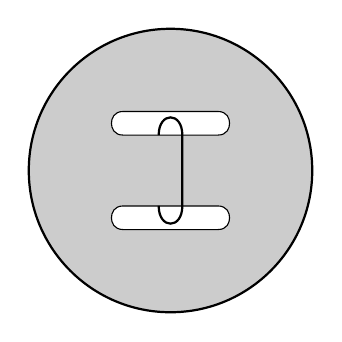
\begin{tikzpicture}[scale=0.6]
\fill[color = black!20] (0, 0) circle (3);
\draw[thick] (0, 0) circle (3);
\draw[fill = white] 
	(-1.25, -1) .. controls +(0, 0.1) and +(-0.2, 0) ..
	(-1, -0.75) --
	(1, -0.75) .. controls +(0.2, 0) and +(0, 0.1) ..
	(1.25, -1) .. controls +(0, -0.1) and +(0.2, 0) ..
	(1, -1.25) --
	(-1, -1.25) .. controls +(-0.2, 0) and +(0, -0.1) ..
	(-1.25, -1);
\draw[fill = white] 
	(-1.25, 1) .. controls +(0, -0.1) and +(-0.2, 0) ..
	(-1, 0.75) --
	(1, 0.75) .. controls +(0.2, 0) and +(0, -0.1) ..
	(1.25, 1) .. controls +(0, 0.1) and +(0.2, 0) ..
	(1, 1.25) --
	(-1, 1.25) .. controls +(-0.2, 0) and +(0, 0.1) ..
	(-1.25, 1);
\draw[thick] 
	(-0.25, -0.75) .. controls +(0, -0.5) and +(0, -0.5) ..
	(0.25, -0.75) --
	(0.25, 0.75) .. controls +(0, 0.5) and +(0, 0.5) ..
	(-0.25, 0.75);
\end{tikzpicture}


\end{document}
